\cia\vspace{-2cm}
\section{Bethe Heitler processes}
\label{sec:bethe} 
\F{fig:wmm_after_fiducial} shows the $(e,P)$ missing mass $M_X^2$ versus $W$ distribution
for the whole e1-6 period after particle ID, vertex fiducial cuts and kinematic corrections.
The elastic and Bethe Heitler (B.H.) events, illustrated in \F{fig:bethe},
are clearly seen at $M_X^2=0$, with the characteristic increase of
the cross section at high $W$. Also shown are the $S_{11}(1535)$ resonance decaying in $\eta$, 
the $P_{13}(1720)$ resonance decaying in $\rho$ and the subject of this analysis, the
$\Delta_{33}(1232)$ resonance decaying in $\pi^0$.

\begin{figure}[h]
 \begin{center}
 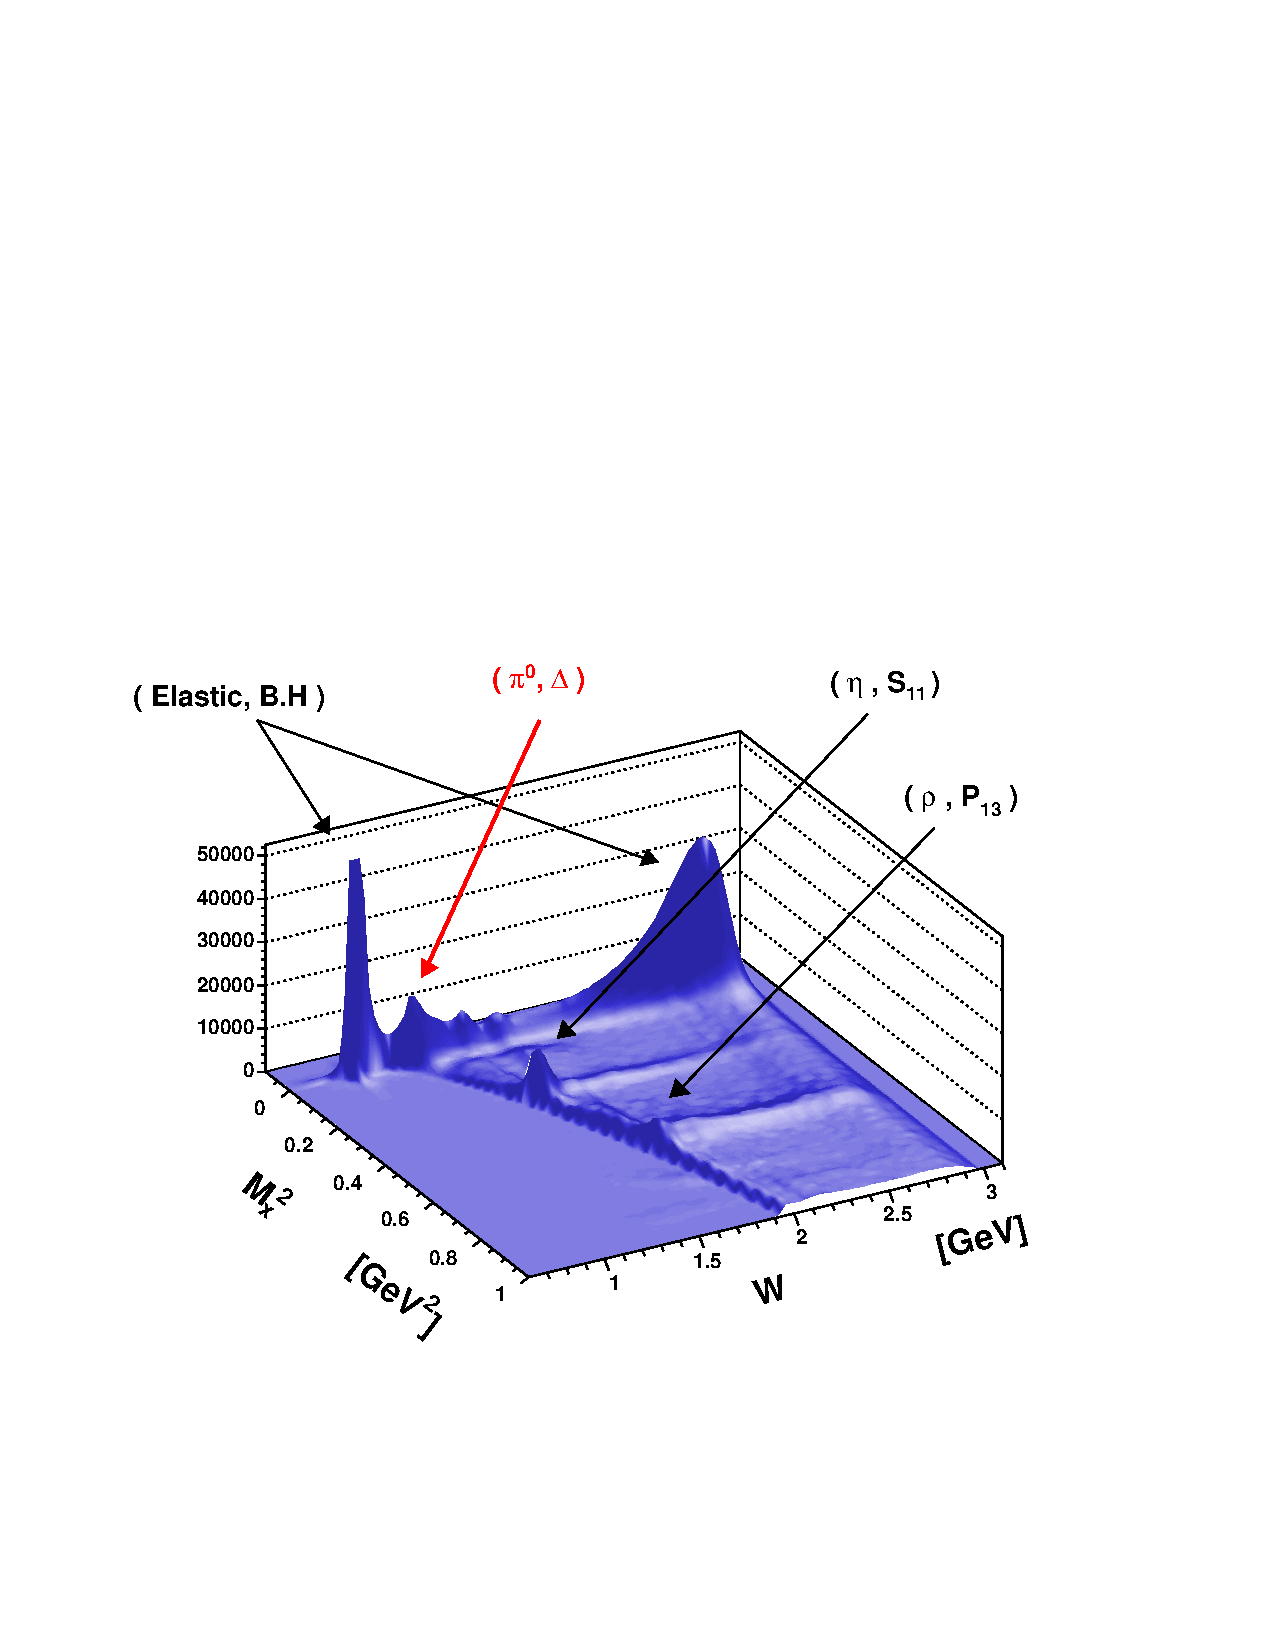
\includegraphics[width = 14cm, bb=0 120 540 540]{data_reduction/img/wmm_after_fiducial}   
  \caption[Missing mass $M_X^2$ versus $W$ after particle ID, vertex fiducial cuts and kinematic corrections for the whole e1-6 data]
          { Missing mass $M_X^2$ versus $W$ after particle ID, vertex fiducial cuts and kinematic 
                     corrections for the whole e1-6 data. Clearly visible are the elastic and B.H. events, the  
		     $S_{11}\rightarrow\eta$, the $P_{13}\rightarrow\rho$ and of course the $\Delta_{33}\rightarrow\pi^0$ events.}
 \label{fig:wmm_after_fiducial}
 \end{center} 
\end{figure}

To isolate the $p(e, e'p)\pi^0$ reaction a missing mass technique alone cannot separate
the B.H. processes from the $\pi^0$ events efficiently because of the limited resolution.
What follows is the investigation of the kinematic cuts used to remove the B.H. events from
the inelastic data.

An important assumption used to identify B.H. events is the so called {\it peaking approximation}. It means that
the direction of the emitted photon in reaction like the ones shown in \F{fig:bethe} a) and b) 
is \underline{the same} as the electron. Therefore the electron does not change direction when radiating a photon, 
although it can change energy. This approximation describes well most electron B.H. events \cite{bib:motsai}.

\begin{figure}[h]
 \begin{center}
 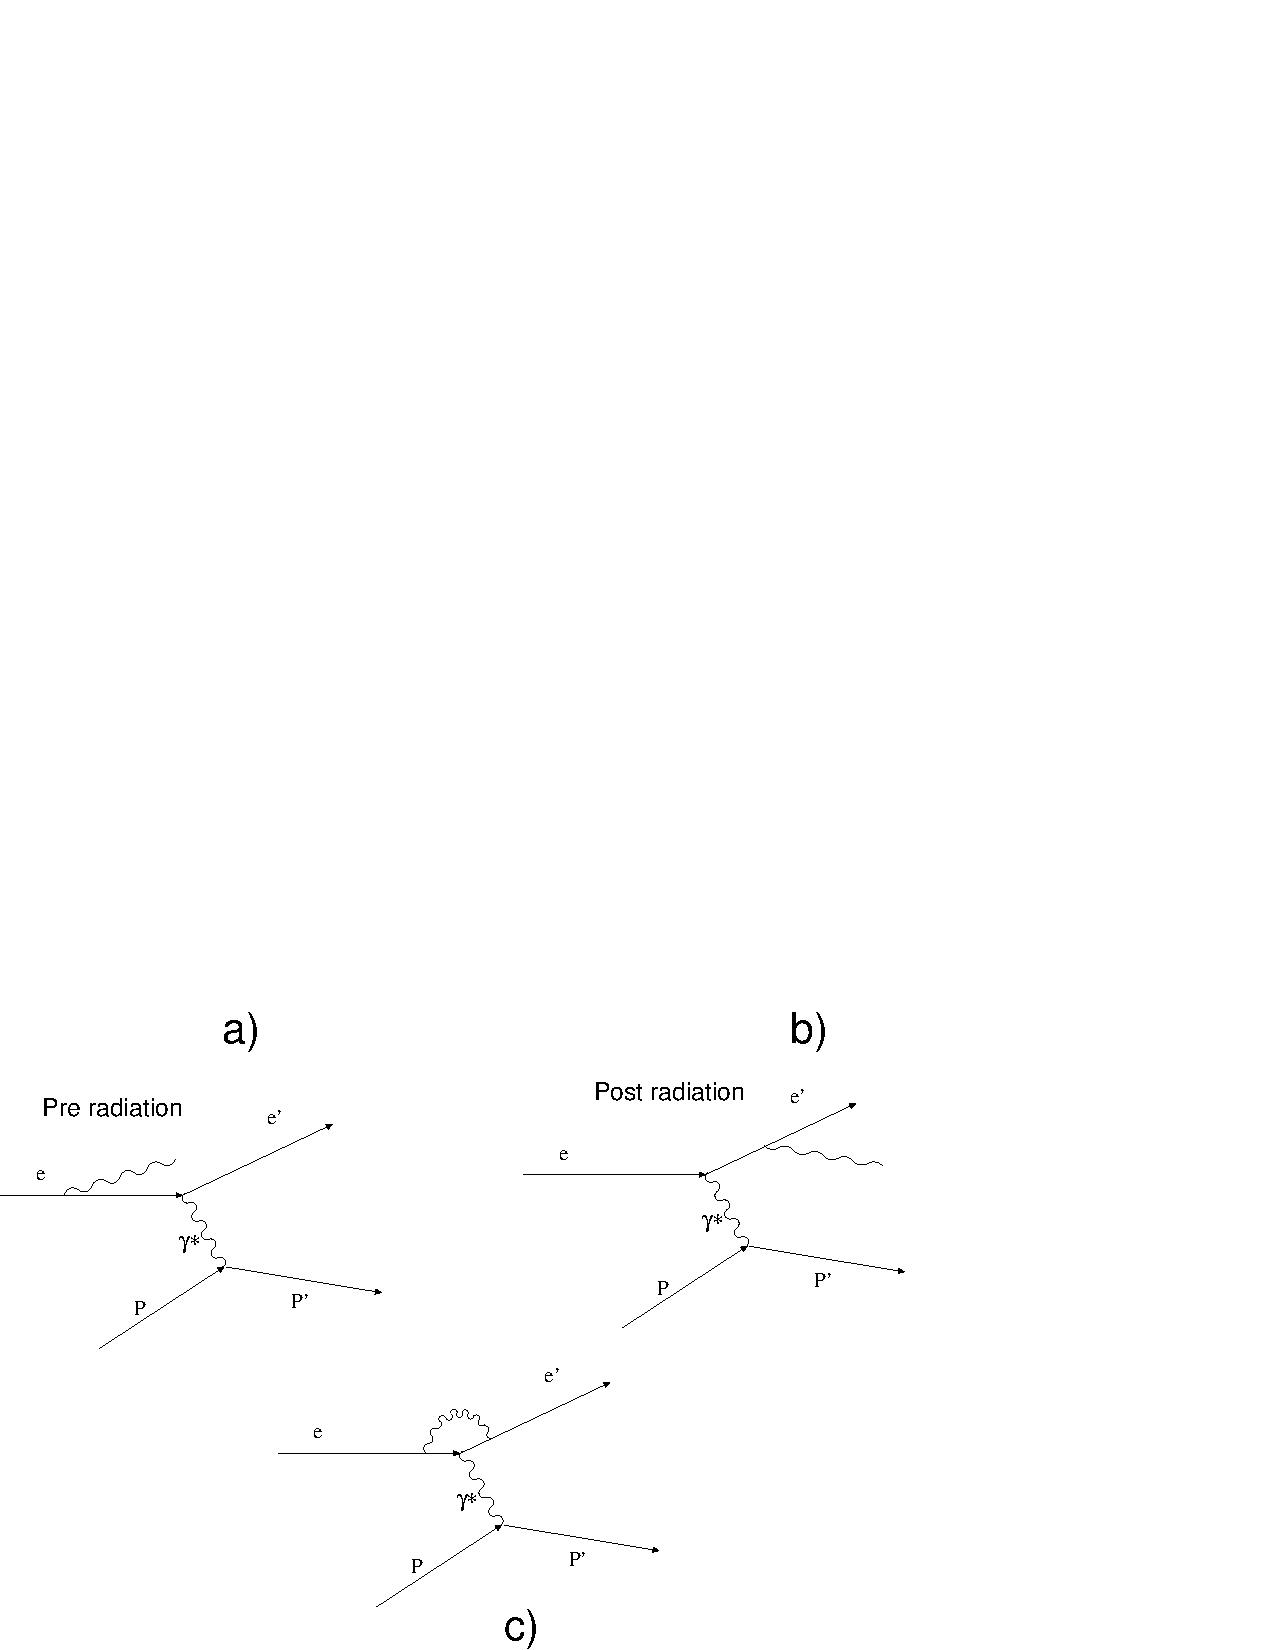
\includegraphics[width = 12cm, bb=-100 -20 570 350]{data_reduction/img/bethe} 
  \caption[Bethe Heitler events contributing to the (eP) final state]
          { Bethe Heitler events contributing to the (eP) final state leaking into
                the $\pi^0$ missing mass.}
 \label{fig:bethe}
 \end{center}
\end{figure}
 
The variables used for the separation are:
\begin{itemize}
 \item {\boldmath $M_x$:} missing mass squared of the final state (eP). 
 
 \item {\boldmath $\Delta\theta = \theta^P_{meas} - \theta^P_{calc}$ :} $\theta^P_{meas}$ is the measured proton angle
                  and $\theta^P_{calc}$ is the proton angle calculated from the outgoing electron energy and angle 
                  (see Section \ref{sec:elastic_selection}). In the peaking approximation, $\Delta\theta$ is  
		  independent of {\bf pre-radiation} processes like the ones in \F{fig:bethe} a) 
		  and it assumes the value zero for elastic and B.H. events.
 
 \item {\boldmath $\Delta\theta_2=\theta^P_{meas} - \theta^P_{calc2}$ :} $\theta^P_{meas}$ is the measured proton angle
                  and $\theta^P_{calc2}$ is the proton angle calculated from the incoming electron energy and 
		  outgoing electron angle (see Section \ref{sec:elastic_selection}). In the peaking approximation, $\Delta\theta_2$ is  
		  independent of {\bf post-radiation} processes line the ones in \F{fig:bethe} b) 
		  and it assumes the value zero for elastic and B.H. events.

 \item{\boldmath $\phi_P^{c.m.}$ :} the azimuthal angle of the proton in the resonance center of mass,  equal 
       to $\pi$ for B.H. events in the peaking approximation.       
\end{itemize}
The contamination is $W$ dependent, so eight bins in $W$ have been considered from $1.08$ to $1.48$ GeV. 
Three cuts have been used in series as described below.

The $\phi_P^{c.m.}$ of the elastic events narrows in $\phi$ and broadens in $M_x^2$ as $W$ increases as 
it is shown in \F{fig:bh_phi_mm} where it is plotted against the missing mass $M_x^2$.
The first cut, represented by the black curve in \F{fig:bh_phi_mm}, is composed by:
\begin{itemize}
 \item A circle whose radius and center vary with $W$.
 \item A hyperbole $y = \pi \pm \Dfrac{a}{x-x_0}$ whose $a$ and $x_0$ vary with $W$.
\end{itemize}

\begin{figure}[h]
 \begin{center}
 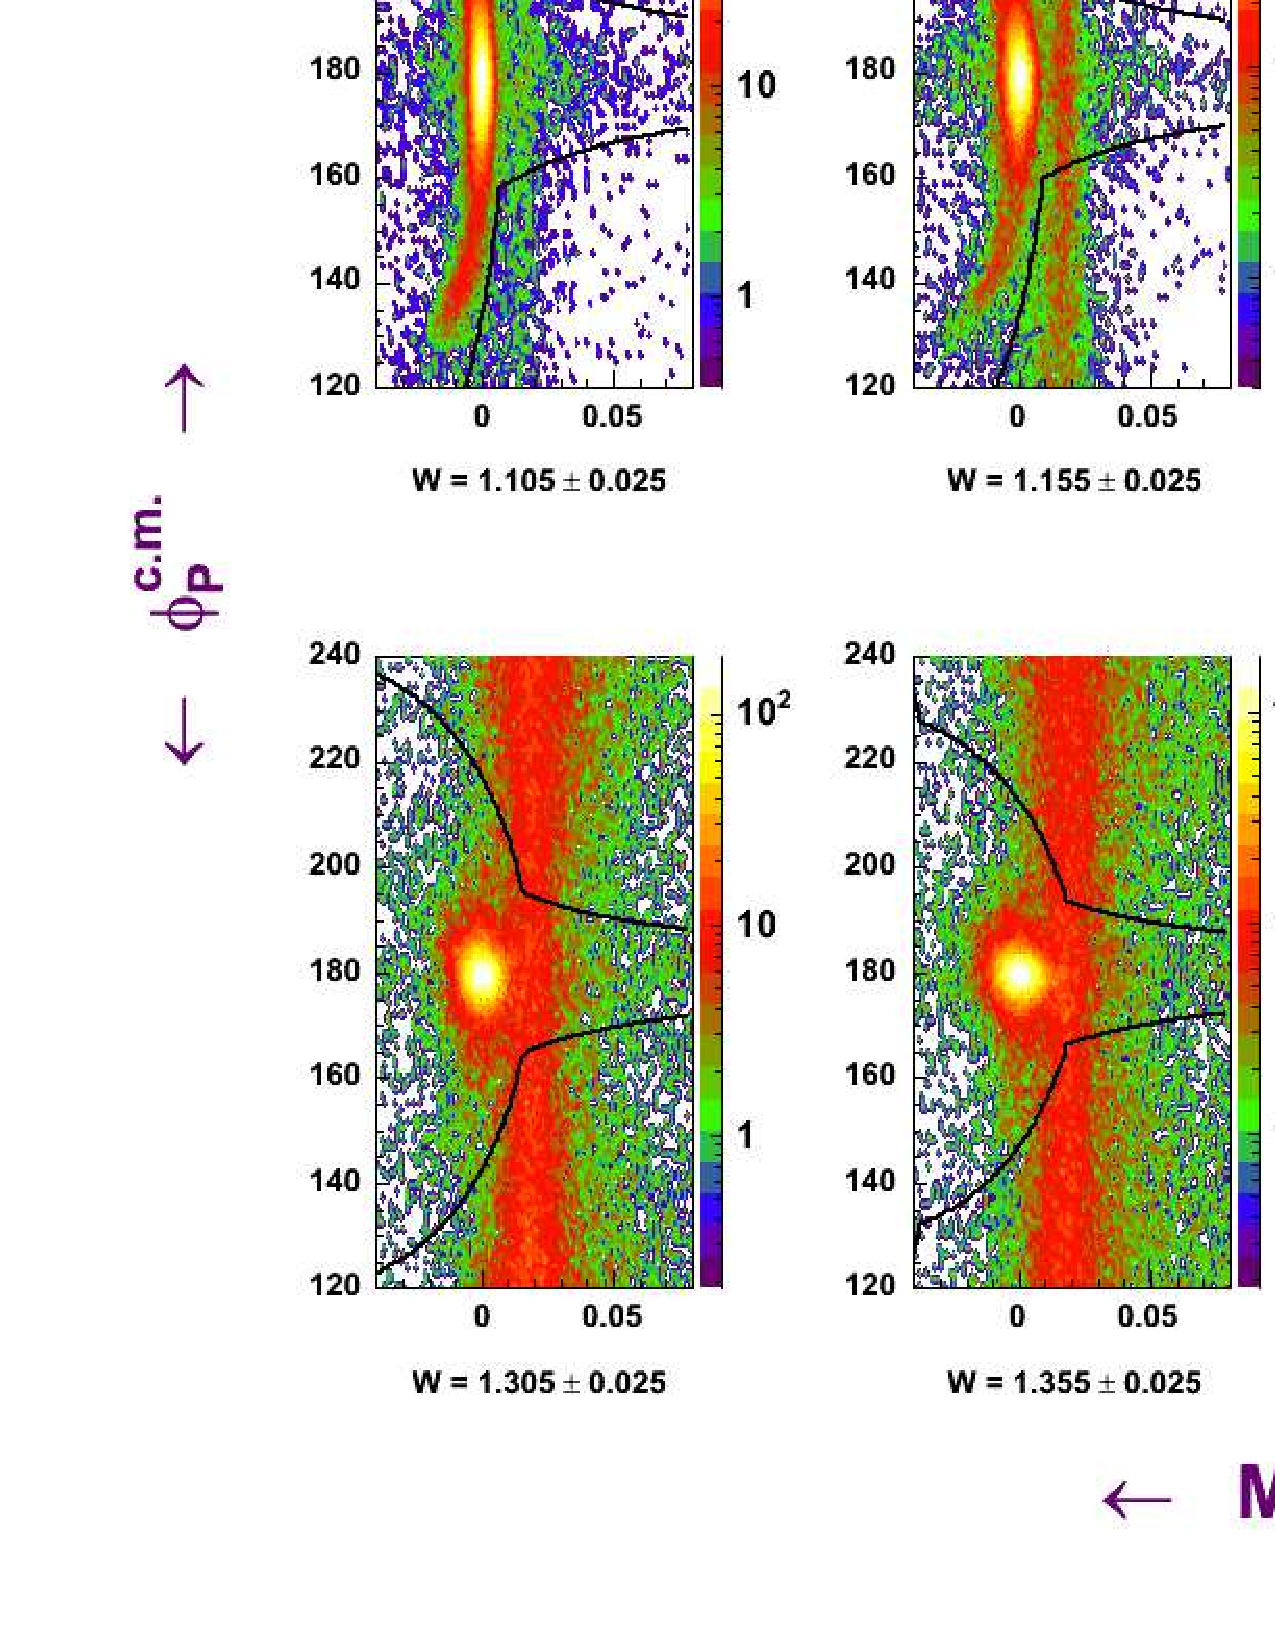
\includegraphics[width = 15.2cm, bb=40 40 1220 940]{data_reduction/img/bh_phi_mm} 
  \caption[$\phi_P^{c.m.}$ versus missing mass $M_x^2$ for different $W$ values]
          { $\phi_P^{c.m.}$ versus missing mass $M_x^2$ for different $W$ values.}
 \label{fig:bh_phi_mm}
 \end{center}
\end{figure}
One can immediately notice that the cut used eliminates some $\pi^0$s around $\phi_P^{c.m.}=180^0$.
These events (and the ones eliminated with the second and third cut below) 
will be recovered with the MonteCarlo simulation because the exact same cut will
be applied (see section \ref{ref:mcbethe}). The closer to data the model used for the simulation, 
the more accurate will be this recovery.

In \F {fig:bh_mm_dth_before} is plot the (eP) missing mass $M_x^2$ versus $\Delta\theta$ distribution.
One can see the pre-radiative events showing at $x=0$ and leaking in the $\pi^0$ events
(horizontal band at $M_x^2\simeq M_{\pi^0}^2=0.0182 $GeV$^2$. The (moving with $W$) spot on the left 
refers to post radiation events.


\begin{figure}[h]
 \begin{center}
 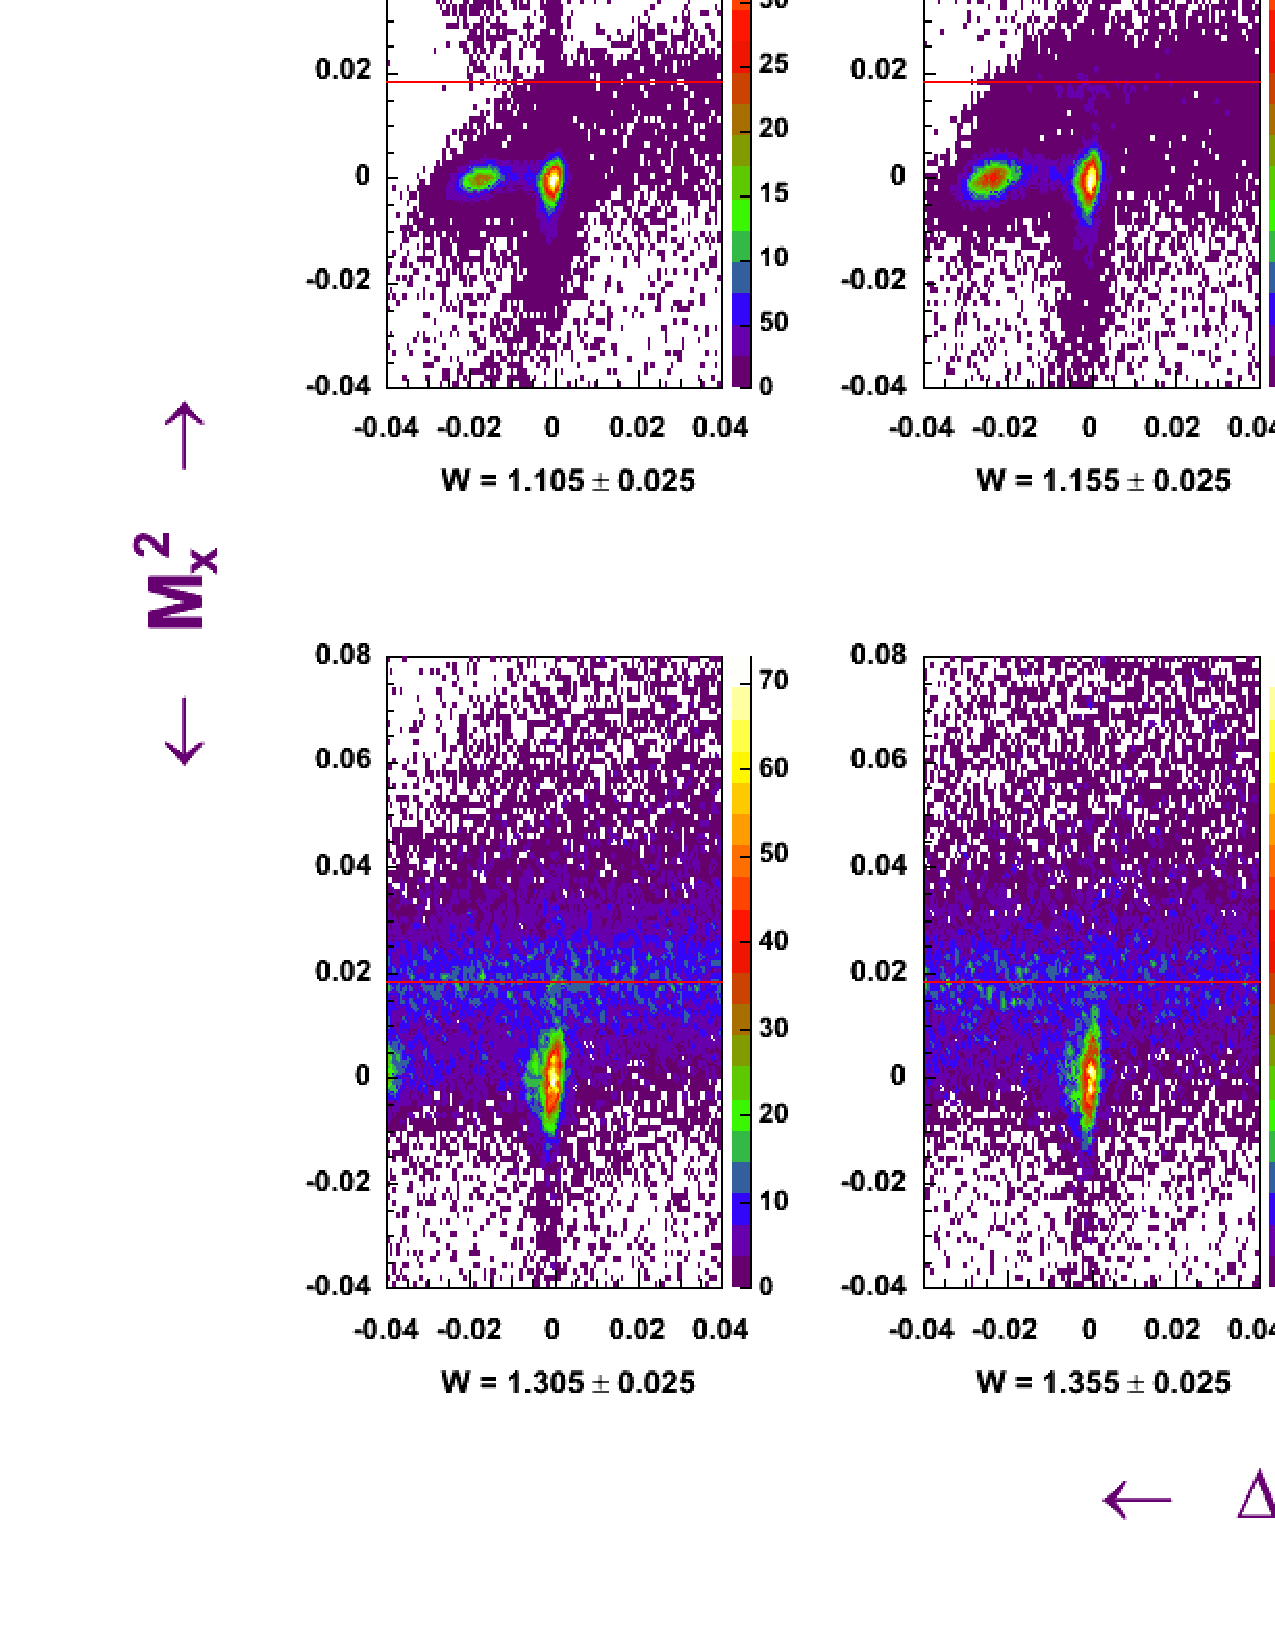
\includegraphics[width = 15.2cm, bb=40 40 1220 1000]{data_reduction/img/bh_mm_dth_before} 
  \caption[missing mass $M_x^2$  versus $\Delta\theta$ for different $W$ values before
          the $\phi_P^{c.m.}$ versus missing mass $M_x^2$ cut]
          { missing mass $M_x^2$  versus $\Delta\theta$ for different $W$ values \underline{before}     the
                     $\phi_P^{c.m.}$ versus missing mass $M_x^2$ cut. The post-radiative 
                     elastic events peak at $x=0$, while the other spot on the left is due to to pre radiation. 
		     The horizontal line is at the $\pi^0$ mass.}
 \label{fig:bh_mm_dth_before}
 \end{center}
\end{figure}
\cia



\begin{figure}[h]
 \begin{center}
 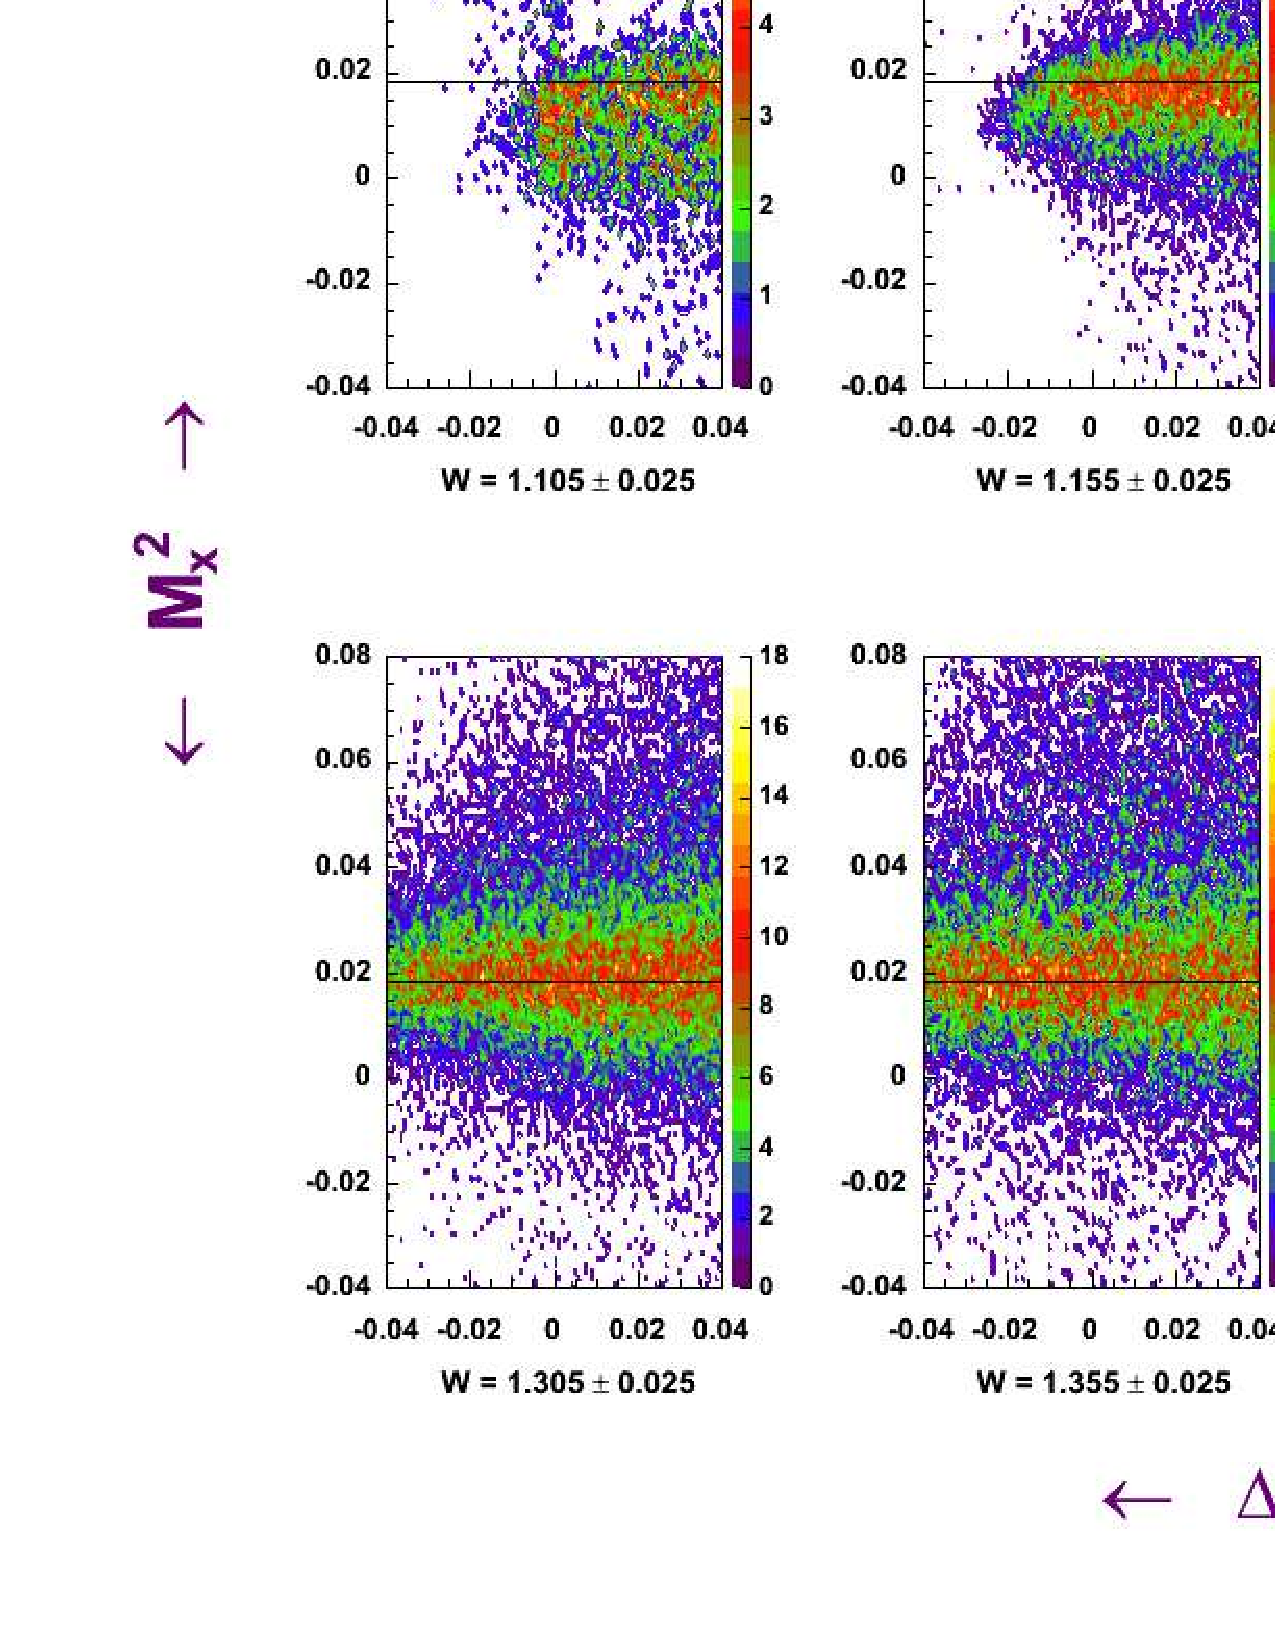
\includegraphics[width = 15.2cm, bb=40 40 1220 1000]{data_reduction/img/bh_mm_dth_after} 
  \caption[missing mass $M_x^2$ versus $\Delta\theta$ for different $W$ values after the $\phi_P^{c.m.}$ versus missing mass $M_x^2$ cut]
          { missing mass $M_x^2$ versus $\Delta\theta$ for different $W$ values \underline{after} the
                     $\phi_P^{c.m.}$ versus missing mass $M_x^2$ cut. 
	             The horizontal line is at the $\pi^0$ mass.}
 \label{fig:bh_mm_dth_after}
 \end{center}
\end{figure}

\F{fig:bh_mm_dth_after} shows the effect of the first cut on the 
missing mass $M_x^2$ versus $\Delta\theta$ distribution. Most of the pre and post radiative events
are eliminated but some residual pre-radiative  B.H. events at low $W$ survives.

For this reason a second cut is introduced:
\begin{equation}
 \label{eqn:second_bh_cut}
 \left| \Delta\theta \right| < 0.01 \,\,{\rm rad} \;\;\;\;\; {\rm when} \;\;\;\;\; W<1.21\,\,{\rm GeV}
\end{equation}
\cia   
Some residual post radiative B.H. events survive the first and second cut. This can be seen in \F{fig:bh_mm_dthb}
where missing mass $M_x^2$ is plotted versus $\Delta\theta_2$: a small band shows up at $\Delta\theta_2\simeq 0$,
particularly at low $W$.\\
The third cut considered, involving missing mass $M_x^2$ versus $\Delta\theta_2$, is:
$$
 M_x^2 < a+b\,\Delta\theta_2
$$
where $a,b$ vary with $W$. 
\begin{figure}[h]
 \begin{center}
 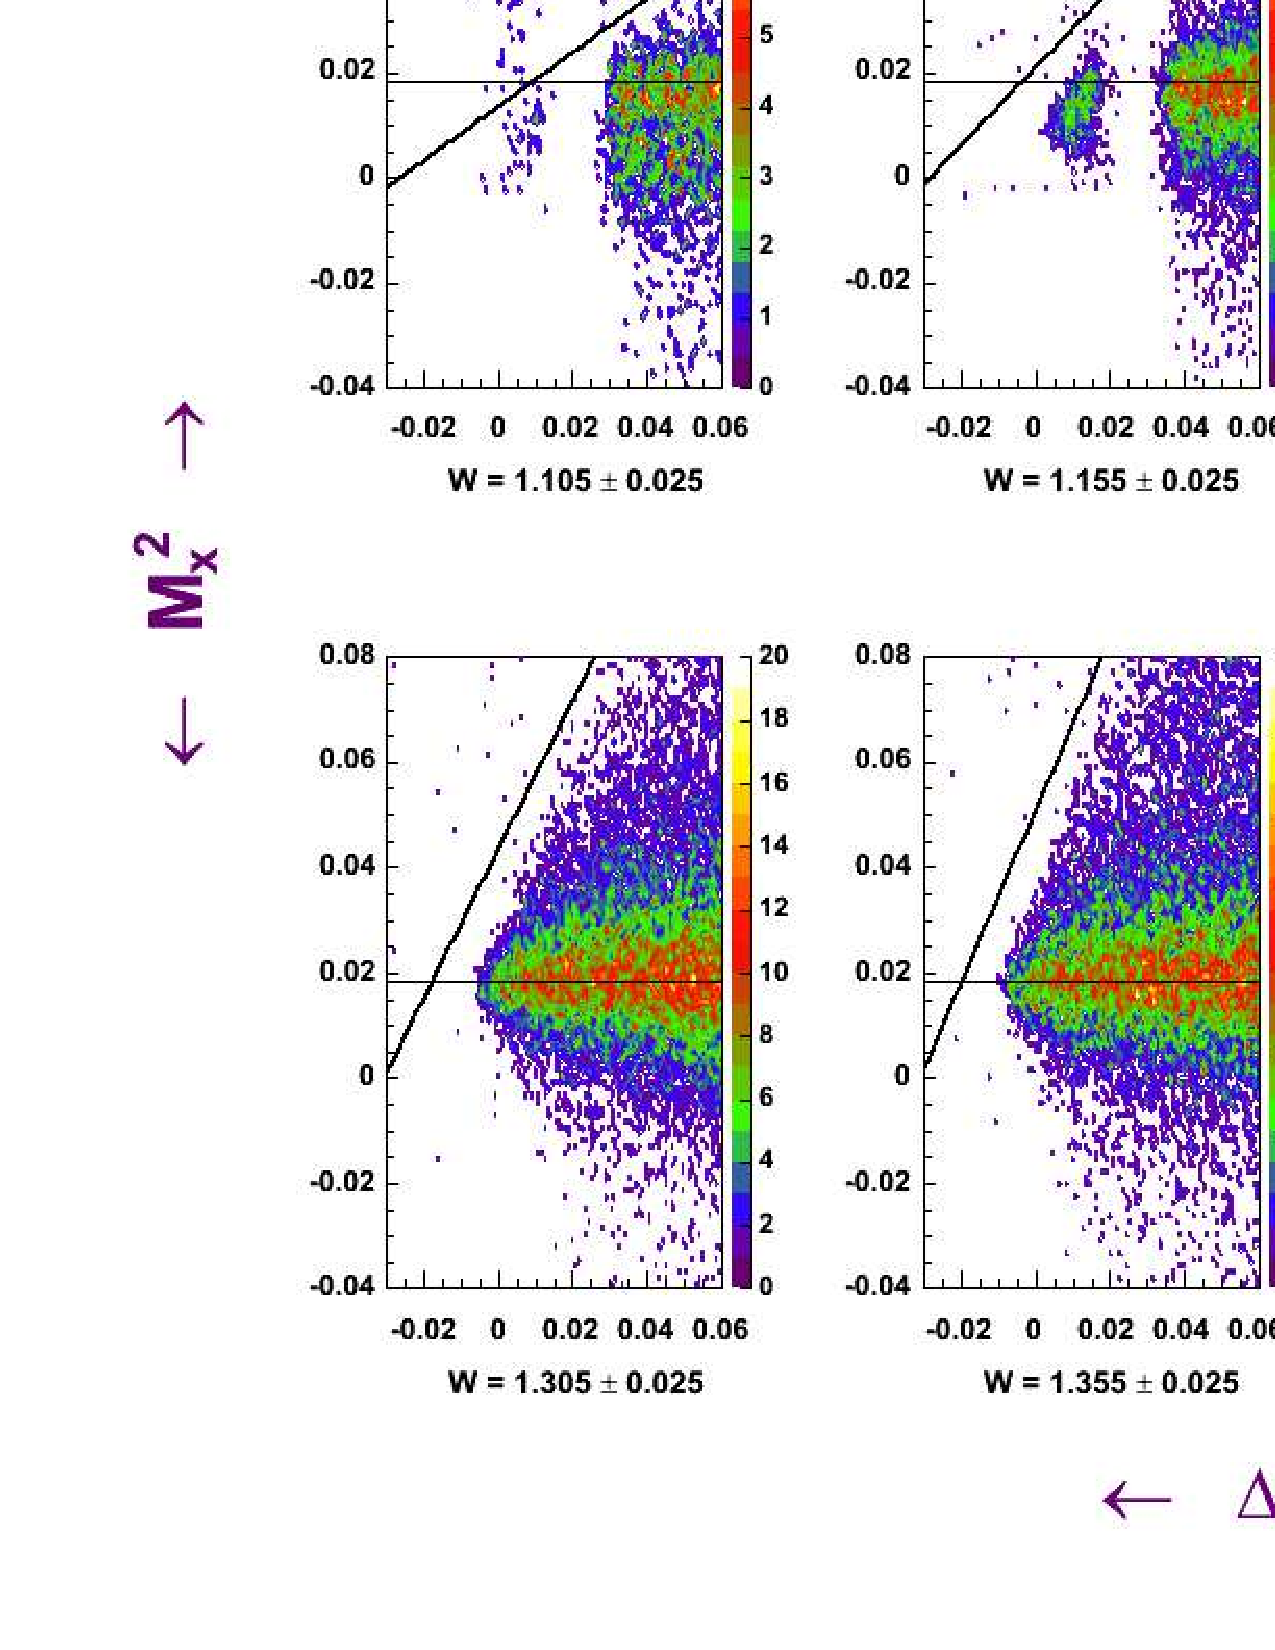
\includegraphics[width = 15cm, bb=0 40 1300 1000]{data_reduction/img/bh_mm_dthb} 
  \caption[missing mass $M_x^2$ versus $\Delta\theta_2$ after the first two B.H. cuts]
          { missing mass $M_x^2$ versus $\Delta\theta_2$ after the first two B.H. cuts.
                     Residual post-radiative events are cut out with a straight line $y=a+bx$ whose 
		     parameters $a$ and $b$ vary with $W$. This plot shows also the effect of
		     the second cut (\ref{eqn:second_bh_cut}): at low $W$ 
		     events with $\Delta\theta\simeq 0\;\equiv\; \Delta\theta_2\simeq 0.025$ disappeared.
		     The horizontal line is at the $\pi^0$ mass.}
 \label{fig:bh_mm_dthb}
 \end{center}
\end{figure}

\cia
After the three cuts described above a ``clean'' sample of $\pi^0$ events is ready for analysis.
This is shown in \F{fig:bh_mm_w} where $W$ and missing mass $M_x^2$ are plotted in blue for the events
surviving the cuts.


\begin{figure}[h]
 \begin{center}
 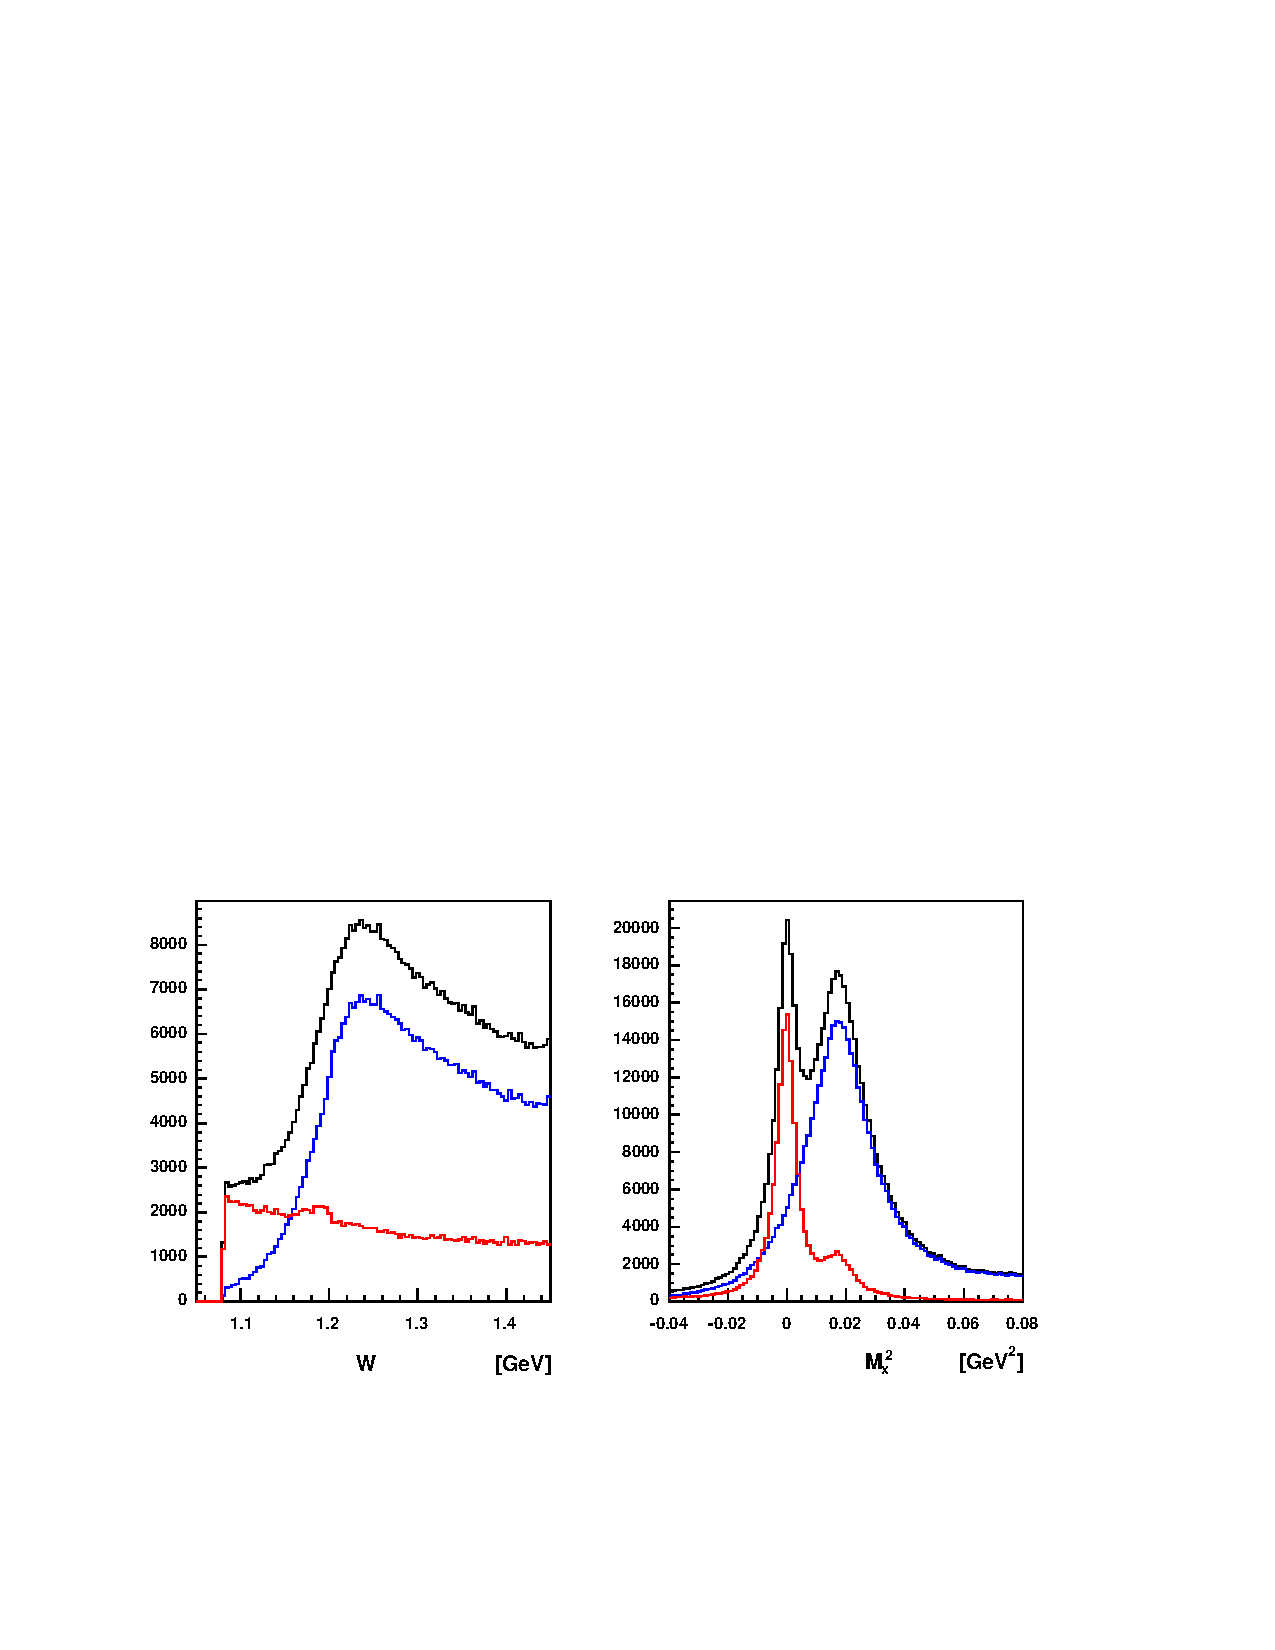
\includegraphics[width = 13cm, bb=60 110 520 460]{data_reduction/img/bh_mm_w} 
  \caption[The effect of all the cuts on the $W$ and missing mass $M_x^2$ distributions]
          { The effect of all the cuts on the $W$ and missing mass $M_x^2$ distributions. 
                     Black line: before any cut. Red line: B.H events. Blue line: final $\pi^0$ events.}
 \label{fig:bh_mm_w}
 \end{center}
\end{figure}












